\documentclass[12pt,a4paper,oneside]{article}
\usepackage[utf8]{vietnam}
\usepackage{amsmath}
\usepackage{amsfonts}
\usepackage{amssymb}
\usepackage{graphicx}
\usepackage[left=2cm,right=2cm,top=2cm,bottom=2cm]{geometry}
\usepackage{array}
\usepackage{fancyhdr}
\pagestyle{fancy}
\renewcommand\thesection{\Roman{section}.}
\renewcommand\thesubsection{\arabic{subsection}.}
\fancyhf{}
\rhead{Week 3}
\lhead{Hoàng Quốc Bảo - 20194484}
\rfoot{Trang \thepage}

\usepackage{listings}
\usepackage{tcolorbox}
\usepackage{color} % tô màu cho code
\definecolor{dkgreen}{rgb}{0,0.6,0}
\definecolor{gray}{rgb}{0.5,0.5,0.5}
\definecolor{mauve}{rgb}{0.58,0,0.82}
\lstset{frame=tb,
  language=[x86masm]Assembler,
  aboveskip=3mm,
  belowskip=3mm,
  showstringspaces=false,
  columns=flexible,
  basicstyle={\small\ttfamily},
  backgroundcolor=\color{gray!20!white},
  numbers=none,
  breaklines=true,
  breakatwhitespace=true,
  tabsize=3
}

\begin{document}
\section{Assignment 1}
\textbf{Mã nguồn:}
\begin{center}
\begin{lstlisting}
#Laboratory Exercise 3, Home Assignment 1
.data 
i : .word 4484
j : .word 2019
.text
start:
la $t4, i	#Load address of i
lw $s1, 0($t4)	#$s1 = i 
la $t4, j	#Load address of j
lw $s2, 0($t4)	#$s2 = j
addi $t1, $zero, 1     #$t1 = x = 1
addi $t2, $zero, 2	#$t2 = y = 2
addi $t3, $zero, 3	#$t3 = z = 3
slt $t0,$s2,$s1 # j<i
bne $t0,$zero,else # branch to else if j<i
addi $t1,$t1,1 # then part: x=x+1
addi $t3,$zero,1 # z=1
j endif # skip "else" part
else: addi $t2,$t2,-1 # begin else part: y=y-1
add $t3,$t3,$t3 # z=2*z
endif:

\end{lstlisting}
\end{center}



\noindent \textbf{Quan sát sự thay đổi của các thanh ghi và các biến:}
\begin{itemize}
\item Khởi tạo giá trị các biến như trong bảng
\begin{center}
\begin{tabular}{|c|c|c|c|c|}
\hline 
i & j & x & y & z \\ 
\hline 
4484 & 2019 & 1 & 2 & 3 \\ 
\hline 
\end{tabular}
\end{center}
\item Sau khi chạy lệnh \quad 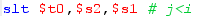
\includegraphics[scale=1]{image/1.1}:\\
\begin{itemize}
\item Sự thay đổi của thanh ghi: 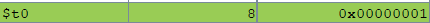
\includegraphics[scale=1]{image/1.2}
\item Giải thích:\\
Lệnh slt thực hiện so sánh 2 thanh ghi \$s2, \$s1. Do \$s2 < \$s1 nên gán thanh ghi \$t0 = 1.
\end{itemize}


\item Sau khi chạy lệnh  \quad 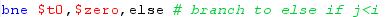
\includegraphics[scale=1]{image/1.3}:\\
\begin{itemize}
\item Giải thích:\\
Lệnh bne thực hiện so sánh bằng nhau giữa thanh ghi \$t0 và \$zero. Do thanh ghi \$t0 
$ \neq $ \$zero nên chương trình sẽ nhảy đến nhãn else.
\end{itemize}

\item Chương trình nhảy đến nhãn else, chạy lệnh \quad 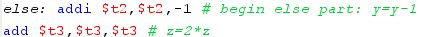
\includegraphics[scale=1]{image/1.4}:\\
\begin{itemize}
\item Sự thay đổi của thanh ghi: 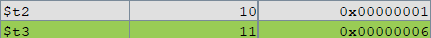
\includegraphics[scale=1]{image/1.5}
\item Giải thích:\\
Lệnh addi thứ nhất thực hiện phép gán \$t2 = \$t2 + (-1) \quad \textbf{(y = y - 1)}\\
Lệnh addi thứ hai thực hiện phép gán \$t3 = \$t3 + \$t3 \quad \textbf{(z = z * 2)}
\end{itemize}
\end{itemize}
\pagebreak
\section{Assignment 2}
\textbf{Mã nguồn:}
\begin{center}
\begin{lstlisting}
#Laboratory 3, Home Assigment 2
.data 
i: .word 0
n: .word 5
step: .word 1
sum: .word 4484
A: .word 1,2,3,4,5 
.text
la $t4, i	#Load i address
lw $s1, 0($t4)	#$s1 = i
la $t4, n	#Load n address
lw $s3, 0($t4)	#$s3 = n
la $t4, step	#Load step address
lw $s4, 0($t4)	#$s4 = step
la $t4, sum	#Load sum address
lw $s5, 0($t4)	#$s5 = sum
la $s2, A	#Load A address
loop: add $s1,$s1,$s4 #i=i+step
add $t1,$s1,$s1 #t1=2*s1
add $t1,$t1,$t1 #t1=4*s1
add $t1,$t1,$s2 #t1 store the address of A[i]
lw $t0,0($t1) #load value of A[i] in $t0
add $s5,$s5,$t0 #sum=sum+A[i]
bne $s1,$s3,loop #if i != n, goto loop
\end{lstlisting}
\end{center}

\noindent \textbf{Quan sát sự thay đổi của các thanh ghi và các biến:}
\begin{itemize}
\item Khởi tạo giá trị các biến như trong bảng
\begin{center}
\begin{tabular}{|c|c|c|c|c|}
\hline 
i & n & step & sum & A[5] \\ 
\hline 
0 & 5 & 1 & 4484 & 1, 2, 3, 4, 5 \\ 
\hline 
\end{tabular} 
\end{center}
\item Sau khi chạy lệnh \quad 
\includegraphics[scale=1]{image/2.2}:\\
\begin{itemize}

\item Sự thay đổi của thanh ghi: 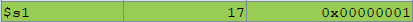
\includegraphics[scale=1]{image/2.3}
\item Giải thích:\\
Lệnh add thực hiện phép gán i = i + step. Do ban đầu i = 0, step = 1 nên sau khi chạy lệnh này, thanh ghi \$s1 sẽ có giá trị = 1.
\end{itemize}


\item Sau khi chạy lệnh \quad 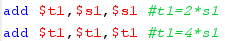
\includegraphics[scale=1]{image/2.4}:\\
\begin{itemize}

\item Sự thay đổi của thanh ghi: 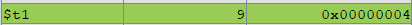
\includegraphics[scale=1]{image/2.5}
\item Giải thích:\\
2 lệnh add này thực hiện phép gán \$t1 = 4 * \$s1. Do 1 word = 4 byte nên mỗi lần muốn trỏ sang 1 phần tử trong mảng word, ta phải tăng biến địa chỉ thêm 4 byte.
\end{itemize}


\item Sau khi chạy lệnh \quad 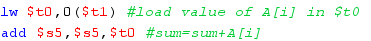
\includegraphics[scale=1]{image/2.6}:\\
\begin{itemize}

\item Sự thay đổi của thanh ghi: 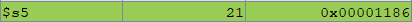
\includegraphics[scale=1]{image/2.7}
\item Giải thích:\\
Lệnh lw sẽ load giá trị của phần tử A[i] vào thanh ghi \$t0. Ở vòng lặp đầu tiên,\\ \$t0 = A[1] = 2.\\
Lệnh add thực hiện phép cộng sum = sum + A[i]. Ở vòng lặp đầu tiên: \\sum = 4484 + 2 = 4486 = 0x1186.

\end{itemize}


\item Sau khi chạy lệnh \quad 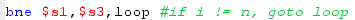
\includegraphics[scale=1]{image/2.8}:\\
\begin{itemize}

\item Giải thích:\\
Lệnh bne thực hiện so sánh i và n. Nếu i $\neq$ n thì sẽ nhảy đến nhãn loop. Cứ như vậy cho đến khi i = n thì chương trình kết thúc.
\end{itemize}

\item Khi chương trình kết thúc, ta thu được kết quả của biến sum:
\begin{center}
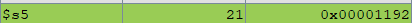
\includegraphics[scale=1]{image/2.9}
\end{center}
\begin{itemize}

\item Giải thích: \\Chương trình kết thúc khi i = n = 5. Khi đó, giá trị của biến sum sẽ là sum = 4484 + A[1] + A[2] + A[3] + A[4] = 4484 + 2 + 3 + 4 + 5 = 4498 = 0x1192.
\end{itemize}
\end{itemize}




\pagebreak
\section{Assignment 3}
\textbf{Mã nguồn:}
\begin{center}
\begin{lstlisting}
#Laboratory Exercise 3, Home Assignment 3
.data
test: .word 1
a: .word 2019
b: .word 4484
.text
la $s0, test #load the address of test variable
lw $s1, 0($s0) #load the value of test to register $s1
la $s0, a #load the address of a variable
lw $s2, 0($s0) #load the value of a to register $s2
la $s0, b #load the address of b variable
lw $s3, 0($s0) #load the value of b to register $s3
li $t0, 0 #load value for test case
li $t1, 1
li $t2, 2
beq $s1, $t0, case_0
beq $s1, $t1, case_1
beq $s1, $t2, case_2
j default
case_0: addi $s2, $s2, 1 #a=a+1
j continue
case_1: sub $s2, $s2, $t1 #a=a-1
j continue
case_2: add $s3, $s3, $s3 #b=2*b
j continue
default:
continue:

\end{lstlisting}
\end{center}
\noindent \textbf{Quan sát sự thay đổi của các thanh ghi và các biến:}
\begin{itemize}
\item Khởi tạo giá trị các biến như trong bảng
\begin{center}
\begin{tabular}{|c|c|c|c|c|c|}
\hline 
test & a & b & \$t0 & \$t1 & \$t2 \\ 
\hline 
1 & 2019 & 4484 & 0 & 1 & 2 \\ 
\hline 
\end{tabular} 
\end{center}

\item Sau khi chạy lệnh \qquad 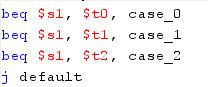
\includegraphics[scale=1]{image/3.2}:\\
\begin{itemize}

\item Giải thích:\\
Đây là một cấu trúc tương trự như switch case.
\begin{itemize}

\item Lệnh beq thứ nhất sẽ so sánh biến test (\$s1) và \$t0. Nếu \$s1 = \$t0 thì sẽ nhảy đến nhãn case\_0.
\item Lệnh beq thứ hai sẽ so sánh biến test (\$s1) và \$t1. Nếu \$s1 = \$t1 thì sẽ nhảy đến nhãn case\_1.
\item Lệnh beq thứ ba sẽ so sánh biến test (\$s1) và \$t2. Nếu \$s1 = \$t2 thì sẽ nhảy đến nhãn case\_2.
\item Nếu không có trường hợp nào thoả mãn, chương trình sẽ nhảy đến nhãn default.
\end{itemize}
Ở trường hợp này, do \$s1 = \$t1 nên chương trình sẽ nhảy đến nhãn case\_1.
\end{itemize}
\end{itemize}




\pagebreak
\section{Assignment 4}
\subsection*{a. i < j}
Để thay đổi điều kiện, ta chỉ cần thay đổi lệnh \lstinline{slt $t0,$s2,$s1 # j<i} thành \lstinline{slt $t0,$s1,$s2 # i<j} là được, giải thích các bước tương tự như Assignment 1.


\subsection*{b. i >= j}
Ta thấy i >= j <=> i < j . Để thay đổi điều kiện, ta chỉ cần thay đổi lệnh \lstinline{slt $t0,$s2,$s1 # j<i} thành \lstinline{slt $t0,$s1,$s2 # i>=j} là được, giải thích các bước tương tự như Assignment 1.






\subsection*{c. i + j <= 0}





\subsection*{d. i + j < m + n}


\pagebreak
\section{Assignment 5}
\subsection*{a. i < n}



\subsection*{b. i <= n}




\subsection*{c. sum >= 0}





\subsection*{d. A[i] == 0}

\pagebreak
\section{Assignment 6}
\textbf{Mã nguồn:}
\begin{center}
\begin{lstlisting}
#Laboratory 3, Home Assigment 6
.data 
A: .word 2, 0, 1, -9, 4, 4, -8, 4		#We will tind the element with the largest absolute value in a list A
.text
la $s2, A	#Load A address
li $s0, 8	#$s0 = Number of element in array (n)aba
li $s1, -1	#default value of i is -1
li $t2, 0	#initial max_abs value is 0
lw $s3, 0($s2)	#initial max abs element is A[0]

loop: addi $s1,$s1,1 	#i=i+1
add $t1,$s1,$s1 #t1=2*s1
add $t1,$t1,$t1 #t1=4*s1
add $t1,$t1,$s2 #t1 store the address of A[i]
lw $t0,0($t1) #load value of A[i] in $t0
abs $t4, $t0	#$t4 is absolute value of A[i]
slt $t3, $t2, $t4	#max abs < abs(A[i])
bne $t3, $zero, else	#branch to else if max < abs(A[i])
j continue
else:
add $t2, $zero, $t4	#max abs = abs(A[i])
add $s3, $zero, $t0	#max abs element = A[i]
continue:
bne $s0, $s1, loop	#if i != n, goto loop


\end{lstlisting}
\end{center}
\textbf{Giải thích:}
\begin{itemize}
\item Khởi tạo các biến:
\begin{itemize}
\item Giá trị mảng A[8] = {2, 0, 1, -9, 4, 4, -8, 4}.
\item Giá trị n = 8 chứa số phần tử của mảng.
\item Khởi tạo biến đếm i = -1. (Mục đích để khi thực hiện lần lặp đầu tiên, lệnh \\\lstinline{addi $s0, $s1, 1} sẽ làm cho i = 0, A[i] sẽ trỏ đến phần tử đầu tiên của mảng.)
\item Khởi tạo giá trị \$t2 = 0 là giá trị max trị tuyệt đối, \$s3 = A[0] là giá trị của phần tử có giá trị tuyệt đối lớn nhất. 
\end{itemize} 
\item Ta lần lượt thực hiện so sánh abs(A[i]) với \$t2. Nếu \$t2 < abs(A[i]) thì \$t2 = abs(A[i]) và \$s3 = A[i].\\
Lặp lại như vậy cho đến khi duyệt qua hết mảng ( i = n ). Giá trị thanh ghi \$s3 chính là giá trị của phần tử có giá trị tuyệt đối lớn nhất.
\end{itemize}

    


\end{document}